\newpage
\section{Container Orchestration Platform -- Kubernetes}
\begin{itemize}
	\item \textbf{Container Orchestration}: management and deployment of lots of containers
	\begin{itemize}
		\item container placement: selection of host for containers
		\item container resource usage monitoring
		\item container health checks
		\item container scaling
		\item access to services: IP management \& load balancing
		\item container networking: microservice communication
		\item persistent storage management
	\end{itemize}
	\item Techniques for container orchestration: \textbf{Kubernetes}, docker, AWS/Azure container service
	\item Kubernetes:
	\begin{itemize}
		\item a \textbf{cluster}: for running application
		\item an \textbf{orchestrator}: run \& coordinate cloud-native \textbf{microservice} applications.
		
		\item \textbf{declarative} management: description of application in \textbf{yaml file}. 
	\end{itemize}
\end{itemize}

\subsection{Kubernetes Architecture and Components}

\begin{figure}[H]
	\centering
	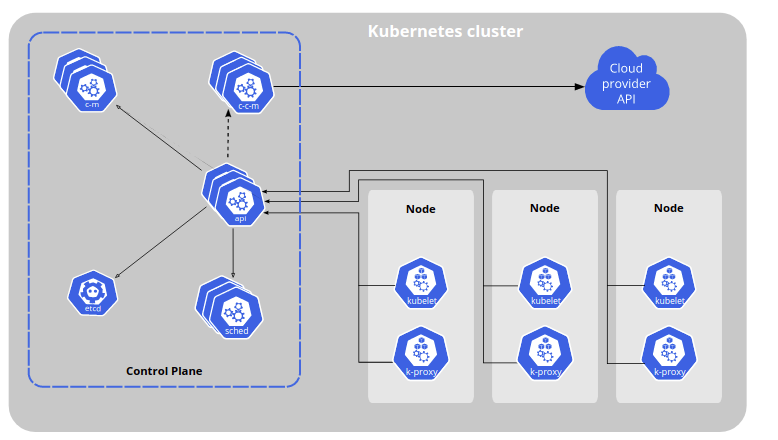
\includegraphics[width=0.8\textwidth]{kubernetes.png}
\end{figure}
\subsubsection{Master Node / Control Plane}
\begin{itemize}
	\item makes \textbf{global decisions} about the cluster as well as \textbf{detecting and responding to cluster events}.
	
	
		\item \textbf{Kube-APIserver}: front-end
		\begin{itemize}
			\item client gateway
			\item REST interface into control plane and datastore.
			\item receives declarative yaml files.
		\end{itemize}
		
		\item \textbf{cluster store}: cluster data key-value storage, consistency over availability. eg: etcd.
		
		\item \textbf{controller manager}: independently control nodes(detect \& restart fail nodes), jobs, endpoints 
		
		\item \textbf{Kube-scheduler}: watches \textbf{newly created pods} with \textbf{no assigned node} and select a node to run on.

\end{itemize}

\subsubsection{Node}
\begin{itemize}

	\item maintains running pods on the node and provides kubernetes runtime environment. 
	\item \textbf{Kubelet}: \textbf{node-level manager} between master and node. 
	\begin{itemize}
		\item receives assignment from Kube-APIserver and report states back.
		\item management of pods lifecycles.
	\end{itemize}
	\item \textbf{container runtime (CRI)}: performs \textbf{container-related tasks}, eg: docker
	\begin{itemize}
		\item pull images, start/stop containers
		\item Each node has only one CRI, different nodes can have different CRIs.
	\end{itemize} 
	\item \textbf{kube-proxy}: local cluster networking, maintain network rules and communication
	\begin{itemize}
		\item ensures each node has \textbf{its own IP}
		\item routing and load-balancing on the pod network for services
	\end{itemize}
\end{itemize}


% Q: each node(eg: a VM) has one pod?
\subsubsection{Pods}
\begin{itemize}
	\item the \textbf{smallest deployable units} of computing that you can \textbf{create and manage} in Kubernetes.
	
	$\rightarrow$ automic unit for starting/stopping/scaling
	
	
	\item Pod: a group of one or more containers, with shared storage and network resources, and a specification for how to run the containers. (resource limits defined in cgroups)
	\item provides environment for containers:
	\begin{itemize}
		\item each pod has a unique IP address.  
		\item each container inside the pod has its own port. 
		\item containers share memory, volumes and network stack. 
	\end{itemize}
	\item pod-to-pod communication: pod network
	\begin{itemize}
		\item bridge network
		\item routing tables
	\end{itemize}
	\item pod deployment:\textbf{declarative description}, provide specification of self-healing(failed pods will be replaced, mortal), scalability and rolling updates. 
	\begin{figure}[H]
			\centering
			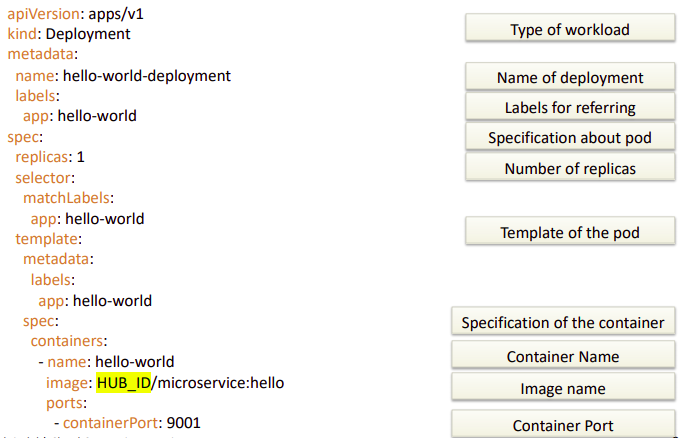
\includegraphics[width=0.8\textwidth]{deployment.png}
	\end{figure}
	\item managed by higher-level controllers:
	\begin{itemize}
		\item deployment
		\item deamonSet
		\item StatefulSet
	\end{itemize}
	
\end{itemize}

\subsection{Service}
\begin{itemize}
	\item provides reliable \textbf{networking for a set of pods}
	\begin{itemize}
		\item stable DNS name, IP address and port 
		\item load balance across a set of pods
	\end{itemize}
	\item types:
	\begin{itemize}
		\item clusterIP service
		\item NodePort service
		\item LoadBalancer service
		\item ExternalName service
	\end{itemize}
	\item service discovery: 
	\begin{itemize}
		\item service \textbf{registers} automatically with \textbf{cluster DNS}. 
		\item request handled by \textbf{rewriting the service IP address} from cluster DNS \textbf{to IP address of pod}.
	\end{itemize}
	
	\begin{figure}[H]
		\centering
		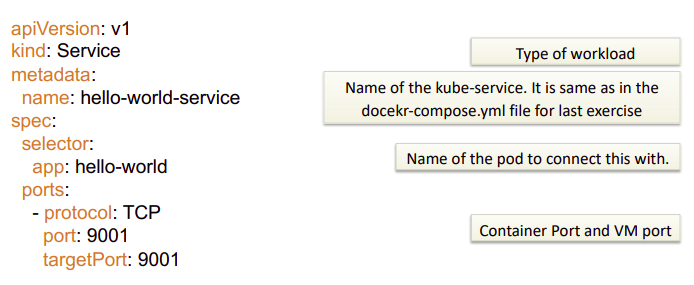
\includegraphics[width=0.8\textwidth]{service.png}
	\end{figure}
\end{itemize}


\subsection{Kubernetes Storage: Persistent Volume}
\begin{itemize}
	\item \textbf{Persistent Volume}: a piece of \textbf{storage in the cluster} that has been provisioned by an administrator or dynamically provisioned using Storage Classes.
	\begin{itemize}
		\item different properties: capacity, storage class, access mode, etc.
		\item persistent volume object : map external storage onto cluster
		\item \textbf{persistent volume claims} (PVC): a request for storage by a user. pods act through PVC to access PV.
		\item storage class: automates creation of PV
	\end{itemize}
\end{itemize}

\subsection{Configuration: ConfigMap}
\begin{itemize}
	\item ConfigMap: stores \textbf{configuration data} outside of a pod, which can be \textbf{dynamically injected into pod at runtime}
	\begin{itemize}
		\item key-value pairs
		\item injected by: environment variables, files in volume, etc.
	\end{itemize}
\end{itemize}

\subsection{Autoscaling \& Monitoring in Kubernetes}

\subsubsection{Autoscaling}
\begin{itemize}
	\item \textbf{horizontal Pod autoscaler}
	\begin{itemize}
		\item modifies number of \textbf{replicaSet}, desired number defined by rules/thresholds
	\end{itemize}
	\item \textbf{vertical Pod autoscaler}
	\begin{itemize}
		\item specification: update policy, resource policy, Deployment/StatefulSet
	\end{itemize}
	\item \textbf{cluster-level autoscaler}: adapts the \textbf{\#nodes}
\end{itemize}

\subsubsection{Monitoring}
\begin{itemize}
	\item Monitoring platform: Prometheus
	\item Monitoring metrics:
	\begin{itemize}
		\item application monitoring: CPU usage, response time
		\item infrastructure monitoring: node monitoring
		\item Kubernetes monitoring: metrics about objects(deployment, pods), apiserver workload, kubelet container metrics
	\end{itemize}
\end{itemize}